\documentclass{article}
\usepackage[utf8]{inputenc}

\title{Tesi}
\author{paolas.serra }
\date{December 2022}
\documentclass[ a4paper, 12pt, oneside]{book}
\usepackage[T1]{fontenc}
\usepackage[utf8x]{inputenc}
\usepackage[english]{babel} 
\usepackage{hyperref}
\usepackage{longtable}
\hypersetup{
    colorlinks=false,
    linkcolor=black,
    filecolor=black,      
    urlcolor=black,
    }

\usepackage[a-1b]{pdfx}  
\urlstyle{same}
\usepackage[utf8]{inputenc}
\pagestyle{plain} % No headers, just page numbers
\pagenumbering{arabic} % Arabic numerals
\setcounter{page}{1}
\usepackage{titling}
\usepackage{graphicx}
\usepackage{xcolor}
\usepackage{lmodern}
\usepackage{float}
\usepackage{titlesec}
\usepackage{lipsum} 
\usepackage{listings}
\usepackage{xcolor}
\usepackage{amsmath}
\usepackage{tikz}
\usetikzlibrary{matrix,chains,positioning,decorations.pathreplacing,arrows}
\usepackage[paper=portrait,pagesize]{typearea}
\titleformat{\chapter}[display]
  {\normalfont\bfseries}{}{0pt}{\Huge}
\newcommand{\subtitle}[1]{%
  \posttitle{%
    \par\end{center}
    \begin{center}\LARGE#1\end{center}
    \vskip0.5em}%
}
% Page Style
\renewcommand{\baselinestretch}{1.5}


% PACCHETTO GEOMETRY PER MARGINI
\usepackage{geometry}
 \newgeometry{
left=   1.5 in,
right=  1.5 in,
}

\usepackage[nottoc]{tocbibind} %per far apparire bibliografia in indice

\begin{document}

\begin{titlepage}
\begin{center}
\begin{figure}[H]
\centering

\includegraphics[width=130mm]{images/tesiSCIENZE_POLITICHE.jpg}
\end{figure}    
\end{center}
\begin{center}
{\Large {Corso di Laurea Magistrale in Data Science and Economics} }
\end{center}
\vspace{0,8 cm}
\begin{center}
{\Large \textsc{title} }
\end{center}
\par
  \vspace{1 cm}
  \begin{flushleft}
  		 \textbf{Relatore}:\\ Prof.ssa Alessandra Micheletti\\
  		 \noindent \textbf{2nd prof}:\\ name surname\\
  \end{flushleft}
\par
  \vspace{0 cm}
  \begin{flushright}
  	\textbf{Candidate}: Paola Serra 
  \end{flushright}
\vspace{0,9 cm}    	  
\vfill
\begin{center}
	{\large Accademic Year 2021/2022}
\end{center}
\end{titlepage}

\break
\tableofcontents
\vspace{1.5cm}
\listoffigures
\vspace{1.5cm}
\listoftables
\break

\newpage
\section{Introduction}
TO BE WRITTEN...
\section{CHAPTER 1}
Data Science and machine-learning industries have grown in prominence in recent years and so the performance of scientific computing always has been, continues to be, and probably always will be crucial.
Nowadays, modern language design and compiler techniques make possible to mostly eliminate the performance trade-off and provide a single environment efficient enough for deploying performance-intensive applications. The Julia programming language fulfills this expectation: provides ease and expressiveness for high-level numerical computing, in the same way as languages such as R, MATLAB, and Python, but also supports general programming. To achieve this, Julia builds upon the lineage of mathematical programming languages, but also borrows much from popular dynamic languages, including Lisp, Perl, Python, Lua, and Ruby.
Work on Julia was started in 2009, by Jeff Bezanson, Stefan Karpinski, Viral B. Shah, and Alan Edelman, who set out to create a free language that was both high-level and fast. Starting from version 0.1.2. in early 2012 to the actual 1.8.3 in December 2022, the language has been downloaded 35 million times, and it was downloaded three times more often in 2021 than in the last three years combined.
It was launched under a liberal MIT license. This means that Julia is an open source language which can be used and/or modified without any right infringement.

Julia is both a dynamically-typed and a static-type language. If a typing mistake occurs, Julia will run the program anyway to output an error message later. 
Although one sometimes speaks of dynamic languages as being "typeless", they are definitely not: every object, whether primitive or user-defined, has a type. The lack of type declarations in most dynamic languages, however, means that one cannot instruct the compiler about the types of values, and often cannot explicitly talk about types at all. In static languages, on the other hand, while one can – and usually must – annotate types for the compiler, types exist only at compile time and cannot be manipulated or expressed at run time. In Julia, types are themselves run-time objects, and can also be used to convey information to the compiler.
The code you write is usually converted into some other form that a computer knows how to run. This process is called compilation, and the period of time this happens is called "compile time".
After compilation is over, the program is launched, and the period it's running is called "runtime".
Statically typed languages check the types and look for type errors during compile time.
Dynamically typed languages check the types and look for type errors during runtime.
Another way to think about it: static typing means checking the types before running the program; dynamic typing means checking the types while running the program.
Partly because of run-time type inference (augmented by optional type annotations) and just-in-time (JIT) compilation, implemented using LLVM, and partly because of a strong focus on performance from the inception of the project, Julia's computational efficiency exceeds that of other dynamic languages, and even rivals that of statically-compiled languages. 
It also features REPL (Read Eval Print Loop), an interactive command-line used to add quick commands and scripts that will read, run, and print out the results of those commands, all in a loop and a fully-featured debugging suite.
It is multi-paradigm, combining features of imperative, functional, and object-oriented programming.  
The core language imposes very little, Julia Base and the standard library are written in Julia itself, including primitive operations like integer arithmetic.
A rich language of types for constructing and describing objects, that can also optionally be used to make type declarations
\subsection{Julia Vs Python }
Python is one of the world's most popular programming languages. Introduced in 1991, it's a high-level, interpreted, general-purpose, multi-paradigm language with an impressive number of libraries and tools dedicated to web and software development, Artificial Intelligence and Machine Learning.
Python's versatility derives from the vast amount of external libraries developed by its extensive community of developers.
The following is a comparison between the Julia programming language and Python:
\begin{itemize}
 \setlength\itemsep{-0.3em}
\item Familiar Syntax: Syntax is simple and easy to understand. Programmers acquainted with Python will be comfortable working with Julia because of their similarities.
\item Call external libraries: Julia can call on different libraries and languages, like Fortran, C, or even Python, allowing data exchange between them.
\item Integration:
Julia can integrate code from Python or C and also use their libraries. Code written in these languages can be converted to Julia, while the opposite is not possible. Julia can also interface directly with Python and share data between both languages.
\item Speed:
Speed is a feature by design in Julia. It is so fast that it is only beaten by C. Python is versatile, powerful but slower, mostly because it's an interpreted language.
Julia is a compiled language that runs just-in-time (JIT) for execution, using the LLVM framework. The written code is compiled to machine code at runtime, delivering higher performance.
\item The ability to define function behavior across many combinations of argument types via multiple dispatch:
Multiple dispatch or multimethods is a feature of some programming languages in which a function or method can be dynamically dispatched based on the run-time (dynamic) type or, in the more general case, some other attribute of more than one of its arguments.
 \end{itemize}

\subsection{Artificial Neural Network}
There are many things computers can do better than humans—calculate square roots or retrieve a web page instantaneously—but our incredible brains are still a step ahead when it comes to common sense, inspiration and imagination. Inspired by the structure of the brain, artificial neural networks (ANN) are the answer to making computers more human like and help machines reason more like humans.
Essentially what each layer of the ANN does is a non-linear transformation of the input from one vector space to another.
Artificial Neural Networks (ANN) are multi-layer fully-connected neural nets that look like the figure below. They consist of an input layer, multiple hidden layers, and an output layer. Every node in one layer is connected to every other node in the next layer. We make the network deeper by increasing the number of hidden layers.

 \begin{figure}[H]
\centering
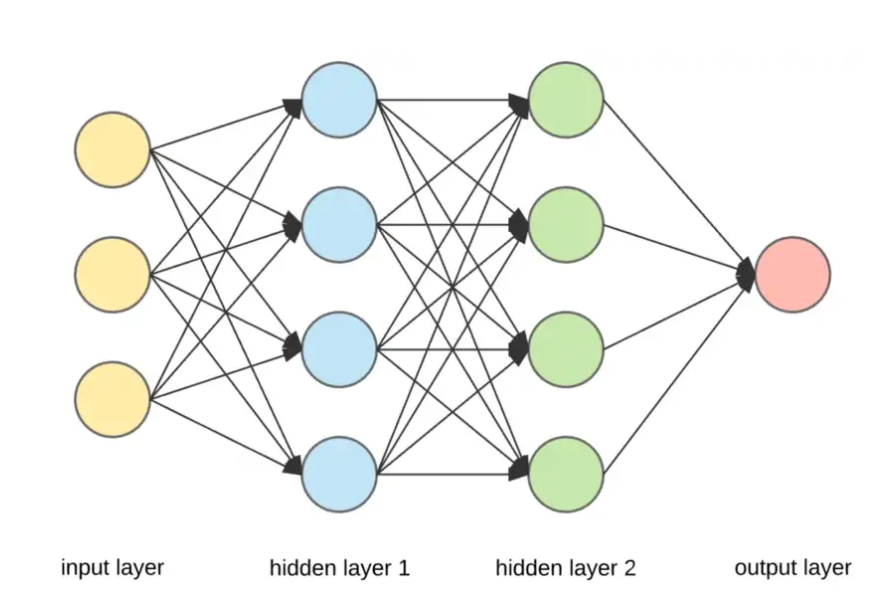
\includegraphics[width=115mm,height=70mm]{images/ann-image.png}
\caption{\label{fig:correlation}Artificial Neural Networks' example with two hidden layers }
\label{6}
\end{figure}
A given node takes the weighted sum of its inputs, and passes it through a non-linear activation function. This is the output of the node, which then becomes the input of another node in the next layer. The signal flows from left to right, and the final output is calculated by performing this procedure for all the nodes. Training this deep neural network means learning the weights associated with all the edges.

 \begin{figure}[H]
\centering
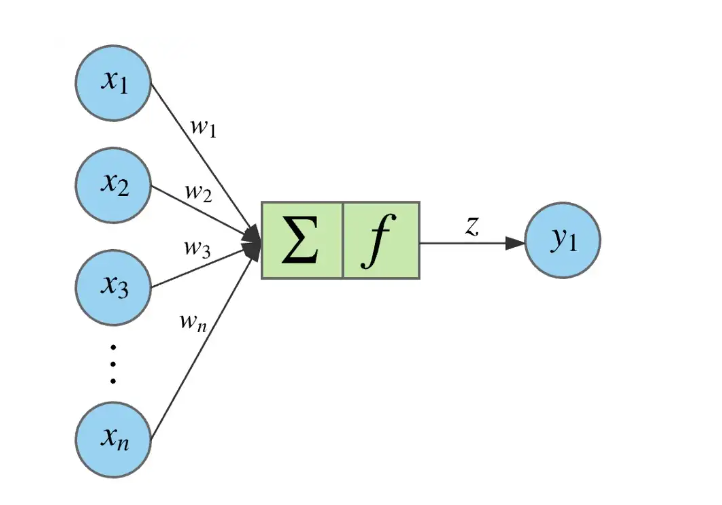
\includegraphics[width=115mm,height=70mm]{images/hidden-layer.png}
\caption{\label{fig:correlation}Forward propagation}
\label{6}
\end{figure}

Putting it all together, the process is summarized in the Figure 3 below:

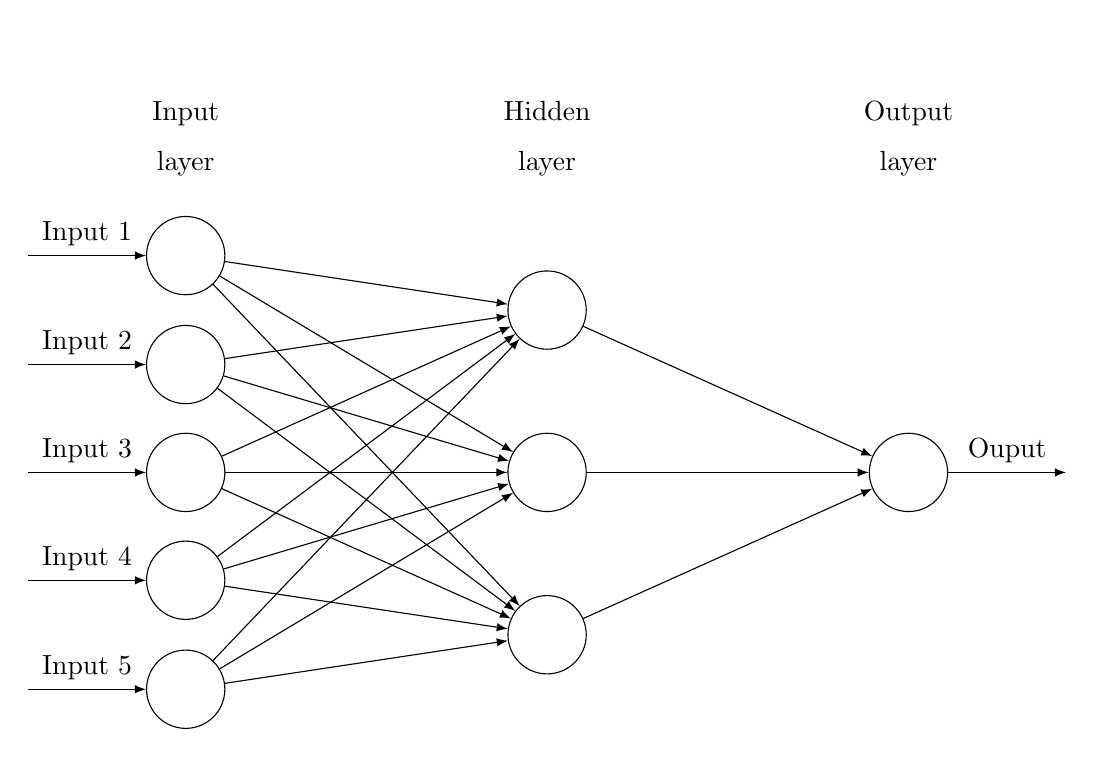
\begin{tikzpicture}[
plain/.style={
  draw=none,
  fill=none,
  },
net/.style={
  matrix of nodes,
  nodes={
    draw,
    circle,
    inner sep=10pt
    },
  nodes in empty cells,
  column sep=2cm,
  row sep=-9pt
  },
>=latex
]
\matrix[net] (mat)
{
|[plain]| \parbox{1.3cm}{\centering Input\\layer} & |[plain]| \parbox{1.3cm}{\centering Hidden\\layer} & |[plain]| \parbox{1.3cm}{\centering Output\\layer} \\
& |[plain]| \\
|[plain]| & \\
& |[plain]| \\
  |[plain]| & |[plain]| \\
& & \\
  |[plain]| & |[plain]| \\
& |[plain]| \\
  |[plain]| & \\
& |[plain]| \\    };
\foreach \ai [count=\mi ]in {2,4,...,10}
  \draw[<-] (mat-\ai-1) -- node[above] {Input \mi} +(-2cm,0);
\foreach \ai in {2,4,...,10}
{\foreach \aii in {3,6,9}
  \draw[->] (mat-\ai-1) -- (mat-\aii-2);
}
\foreach \ai in {3,6,9}
  \draw[->] (mat-\ai-2) -- (mat-6-3);
\draw[->] (mat-6-3) -- node[above] {Ouput} +(2cm,0);
\end{tikzpicture}

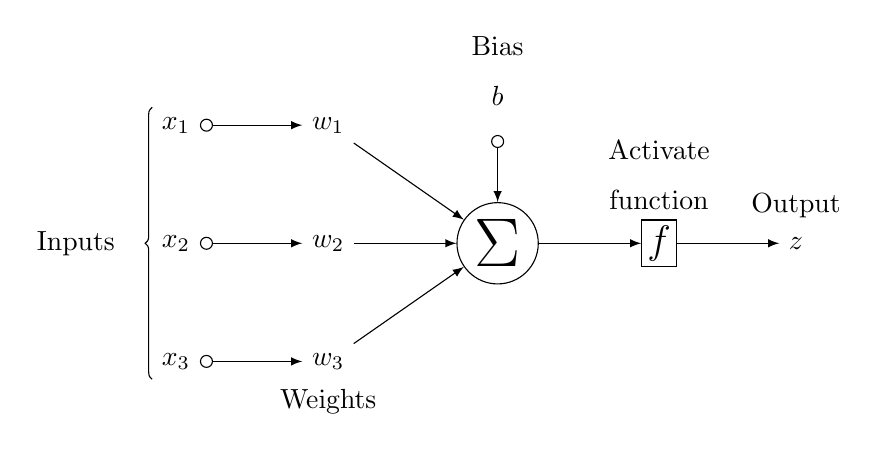
\begin{tikzpicture}[
init/.style={
  draw,
  circle,
  inner sep=2pt,
  font=\Huge,
  join = by -latex
},
squa/.style={
  draw,
  inner sep=2pt,
  font=\Large,
  join = by -latex
},
start chain=2,node distance=13mm
]
\node[on chain=2] 
  (x2) {$x_2$};
\node[on chain=2,join=by o-latex] 
  {$w_2$};
\node[on chain=2,init] (sigma) 
  {$\displaystyle\Sigma$};
\node[on chain=2,squa,label=above:{\parbox{2cm}{\centering Activate \\ function}}]   
  {$f$};
\node[on chain=2,label=above:Output,join=by -latex] 
  {$z$};
\begin{scope}[start chain=1]
\node[on chain=1] at (0,1.5cm) 
  (x1) {$x_1$};
\node[on chain=1,join=by o-latex] 
  (w1) {$w_1$};
\end{scope}
\begin{scope}[start chain=3]
\node[on chain=3] at (0,-1.5cm) 
  (x3) {$x_3$};
\node[on chain=3,label=below:Weights,join=by o-latex] 
  (w3) {$w_3$};
\end{scope}
\node[label=above:\parbox{2cm}{\centering Bias \\ $b$}] at (sigma|-w1) (b) {};

\draw[-latex] (w1) -- (sigma);
\draw[-latex] (w3) -- (sigma);
\draw[o-latex] (b) -- (sigma);

\draw[decorate,decoration={brace,mirror}] (x1.north west) -- node[left=10pt] {Inputs} (x3.south west);


\end{tikzpicture}



 \begin{figure}[H]
\centering
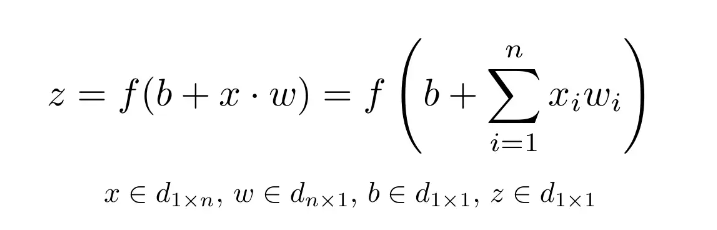
\includegraphics[height=40mm]{images/ann-formula.png}
\caption{\label{fig:correlation}How a neural network works }
\label{6}
\end{figure}
\noindent
There are many types of neural networks available or that might be in the development stage, but we are going to discuss the following three:
\begin{itemize}
 \setlength\itemsep{-0.3em}
\item Multilayer Perceptron:
every single node is connected to all neurons in the next layer which makes it a fully connected neural network. Input and output layers are present having multiple hidden Layers i.e. at least three or more layers in total and it is  is a special case of a feedforward neural network.
Due to the presence of dense fully connected layers and back propagation Multi-Layer Perceptron are used for deep learning, while the main disadvantages are that they are comparatively complex to design and maintain and slow (depends on number of hidden layers).
Examples of MLPs are shown in the figures above.

\item Convolution neural network: contains a three-dimensional arrangement of neurons instead of the standard two-dimensional array. The first layer is called a convolutional layer. Each neuron in the convolutional layer only processes the information from a small part of the visual field. Input features are taken in batch-wise like a filter. The network understands the images in parts and can compute these operations multiple times to complete the full image processing. Processing involves conversion of the image from RGB or HSI scale to grey-scale. Furthering the changes in the pixel value will help to detect the edges and images can be classified into different categories.
Propagation is uni-directional where CNN contains one or more convolutionallayers followed by pooling and bidirectional where the output of convolution layer goes to a fully connected neural network for classifying the images. Filters are used to extract certain parts of the image. In MLP the inputs are multiplied with weights and fed to the activation function. Convolution uses RELU and MLP uses nonlinear activation function followed by softmax. Convolution neural networks show very effective results in image and video recognition, semantic parsing and paraphrase detection.
The main advantages of Convolution Neural Network is the usage of less parameters to learn as compared to fully connected layer

 \begin{figure}[H]
\centering
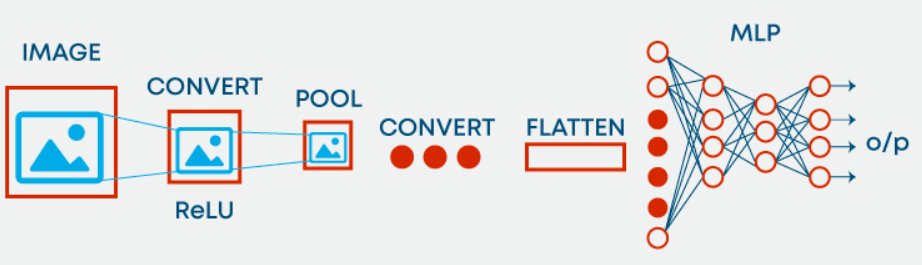
\includegraphics[height=32mm]{images/convolutional.png}
\caption{\label{fig:correlation}Convolution neural network}
\label{6}
\end{figure}

\item  Recurrent Neural Network:
designed to save the output of a layer, RNN is fed back to the input to help in predicting the outcome of the layer. The first layer is typically a feed forward neural network followed by recurrent neural network layer where some information it had in the previous time-step is remembered by a memory function. Forward propagation is implemented in this case. It stores information required for it’s future use. If the prediction is wrong, the learning rate is employed to make small changes. Hence, making it gradually increase towards making the right prediction during the backpropagation.
RNNs can find complex patterns in the input time series and 
can model sequence of data so that each sample can be assumed to be dependent on previous ones.
The disadvantages of Recurrent Neural Networks are the gradient vanishing and exploding problems and the computational difficulties to train recurrent neural nets.



\end{itemize}
 \begin{figure}[H]
\centering
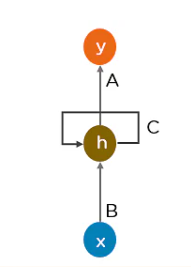
\includegraphics[height=40mm]{images/rnn.png}
\caption{\label{fig:correlation} Recurrent Neural Network }
\label{6}
\end{figure}
\newpage
\noindent

Regardless of the structure of the neural network, each training input is loaded into the neural network in a process called forward propagation. Once the model has produced an output, this predicted output is compared against the given target output in a process called backpropagation, until the hyperparameters of the model are  adjusted so that it  outputs a result closer to the target output.
Neural networks are trained using stochastic gradient descent and require that you choose a loss/cost function when designing and configuring your model.
There are many functions that could be used to estimate the error of a set of weights in a neural network depending on your problem (Cross-entropy , MSE, MAE, etc...).
The gradient descent algorithm  computes the gradient of the loss function for every single weight by the chain rule and seeks to change the weights 
 based on the error rate obtained in the previous epoch (i.e., iteration), meaning that the optimization algorithm is navigating down the gradient (or slope) of error; so that the next evaluation reduces the error making the model reliable by increasing its generalization.

aggiungere qualcosa in più?



ESPANDERE RECURRENT VISTO CHE LE USO
\section{Parametric Machine}

Artificial neural networks and
their architectures can be formally described as particular cases of a general
mathematical construction—machines off finite depth. Unlike neural
networks, machines have a precise definition, from which several properties
follow naturally. Machines of finite depth are modular (they can be
combined), efficiently computable and differentiable. The backward pass
of a machine is again a machine and can be computed without overhead
using the same procedure as the forward pass. We prove this statement
theoretically and practically, via a unifed implementation that generalizes
several classical architectures—dense, convolutional, and recurrent neural
networks with a rich shortcut structure—and their respective backpropagation.



The neural networks explained above are only a subset of all the possible combinations one can choose from, since modern neural networks can have the most diverse structures and do not obey a precise mathematical definition.
In order to define a deep neural network, two solutions have been proposed:
\begin{enumerate}
\item   Combine pre-built layers
\item A differentiable programming approach
\end{enumerate}

The first one allows user to configure the
model via a simplified domain-specific language. It also leads to computationally efficient models, as the rigid structure of the program makes its optimization easier for the library’s software developers.
But it can  become limiting and prevent users from exploring more innovative architectures.

The second one refers to a programming model where
neural networks are truly functional blocks with data-dependent branches and recursion, while at the same time being trainable with backpropagation and gradient descent.
A Differentiable Programming system  is able to take gradients of Julia programs making Automatic Differentiation a first class language
feature.
 Automatic differentiation (AD) is a set of techniques to evaluate the derivative of a function specified by a computer program. AD exploits the fact that every computer program, no matter how complicated, executes a sequence of elementary arithmetic operations (addition, subtraction, multiplication, division, etc.) and elementary functions (exp, log, sin, cos, etc.). By applying the chain rule repeatedly to these operations, derivatives of arbitrary order can be computed automatically, accurately to working precision, and using at most a small constant factor more arithmetic operations than the original program.


This has led to a number of technological advances, ranging from differentiable ray-tracers to neural-network-based solvers for partial differential equations, but unfortunately, it has several drawbacks, some practical and some theoretical. On the practical side, it becomes difficult to optimize the runtime of
the forward and backward pass of an automatically-differentiated code.
The space of models becomes somewhat ill-defined, as it is now the space of all differentiable codes. This concern is not exclusively
theoretical. A well-behaved smooth space of neural networks would
be invaluable for automated differentiable architecture search, where the
optimal network structure for a given problem is found automatically. 
The ambition is to establish a unified framework for deep learning, in
which deep feedforward and recurrent neural networks, with or without shortcut connections, are defined in terms of a unique layer, which we will refer to as a parametric machine. This approach allows for extremely simplified flows for designing neural architectures, where a small set of hyperparameters determines the whole architecture.

\noindent
We start by setting the mathematical foundations for the study of machines.
In order to retain two key notions that are pervasive in deep learning—linearity
and differentiability—we choose to work with normed vector spaces and Fréchet derivatives. We then proceed to build network-like architectures starting from continuously differentiable maps of normed vector spaces.

We start by formalizing how, in the classical deep learning framework, different layers are combined to form a network. Intuitively, function composition
appears to be the natural operation to do so. A sequence of layers

\[X_0 \xrightarrow{l_1} X_1 \xrightarrow{l_2}... X_d_-_1 \xrightarrow{l_d} X_d\]
\noindent
is composed into a map $X_0$ \rightarrow $X_d$. 
We denote composition by juxtaposing
functions:
\[l_d l_d_-_1 ... l_2 l_1:X_0\rightarrow X_d \]
However, this intuition breaks down in the case of shortcut connections or more
complex, non-sequential architectures.
From a mathematical perspective, a natural alternative is to consider a global
space X = \bigoplus $X_i$
and the global endofunction




\begin{equation}
\textit{f}= \sum_{i=1}^{d} l_i \in C^{1} (X,X)
\end{equation}
assume that the output of the network is the entire space X, and not only the output of the
4
last layer, Xd. Let the input function be the continuously differentiable inclusion
map \textit{g} $ \in $  $C^{1} (X_0,X)$. The map g embeds the input data into an augmented
space, which encompasses input, hidden layers, and output. The network transforms the input map g into an output map \textit{h} $ \in $  $C^{1} (X_0,X)$. From a practical
perspective, h computes the activation values of all the layers and stores not
only the final result, but also all the activations of the intermediate layers.
The key observation, on which our framework is based, is that f (the sum of
all layers, as in eq. (1)) and g (the input function) alone are sufficient to determine
h (the output function). Indeed, h is the only map in C1(X0;X) that respects
the following property:

\begin{equation}
\textit{h = g+fh}
\end{equation}
\noindent
There, composition of layers is replaced by their sum. Layers
are no longer required to be sequential, but they must obey a weaker condition of independence.
The existence of a unique solution to eq. (2) for any choice of input function g is the minimum requirement to ensure a well-defined input-output mapping for general architectures.
It will be the defining property of a machine, our generalization of a feedforward deep neural network.

SPIEGAZIONE MATEMATICA: QUANTO ENTRO NEL DETTAGLIO?




\section{Case study}
spiegazione dataset + applicazione parametric machine + risultati

\section{Conclusion}

  
\chapter{}





\begin{thebibliography}{9}





\bibitem{1}{}
https://www.forbes.com/sites/bernardmarr/2018/09/24/what-are-artificial-neural-networks-a-simple-explanation-for-absolutely-anyone/

https://towardsdatascience.com/applied-deep-learning-part-1-artificial-neural-networks-d7834f67a4f6

https://www.mygreatlearning.com/blog/types-of-neural-networks/

https://www.imaginarycloud.com/blog/julia-vs-python/

https://machinelearningmastery.com/loss-and-loss-functions-for-training-deep-learning-neural-networks/


 \end{thebibliography}
    
\lstinputlisting

\end{document}